\chapter{Numeri razionali assoluti}
\label{cha:NumeriRazionaliAssoluti}
\minitoc
\mtcskip                                % put some skip here
\minilof                                % a minilof
\mtcskip                                % put some skip here
\minilot
\section{Frazione}
\label{sec:fraczioniNumRazASS}
Una frazione\index{Numeri!Razionali } è il quoziente\index{Quoziente} di una divisione. Alla frazione $\dfrac{a}{b}$ corrisponde la divisione $a\div b$ e viceversa.
\[
\text{Frazione}=
\dfrac{\text{Numeratore}}{\text{Denominatore}}
\]
Una frazione è\begin{itemize}
	\item Propria\index{Frazione!propria}: il numeratore è minore del denominatore. Es. $\dfrac{2}{3}$ e $\dfrac{7}{8}$
	\item Impropria\index{Frazione!impropria}: il numeratore è maggiore del denominatore. Es. $\dfrac{3}{2}$ e $\dfrac{8}{7}$.
	
	Una frazione impropria può essere scritta come somma di un numero intero e di una frazione propria. 
	
	Esempio: $\dfrac{12}{5}=\dfrac{10}{5}+\dfrac{2}{5}=2+\dfrac{2}{5}$ 
	\item Apparente\index{Frazione!apparente}: il numeratore è un multiplo del denominatore. In questo caso la frazione coincide con un numero intero. Es. $\dfrac{8}{4}$ e $\dfrac{10}{5}$
\end{itemize}
\section{Numeri decimali}
\label{Numeri decimali}
\begin{tikzpicture}[very thick,node distance=5cm,text centered,minimum size=3cm,->=latex]
\node [circle, draw] (a) {Frazione};
\node [circle, draw] (b) [above right=of a] {Numero decimale};
\node [circle, draw] (c) [above left=of a]{Percentuale};
\draw [<->] (a) to (b);
\draw [<->] (b) to (c);
\draw [<->] (c) to (a);
\end{tikzpicture}
\subsection{Da frazione a numero decimale}
\begin{figure}
	\centering
	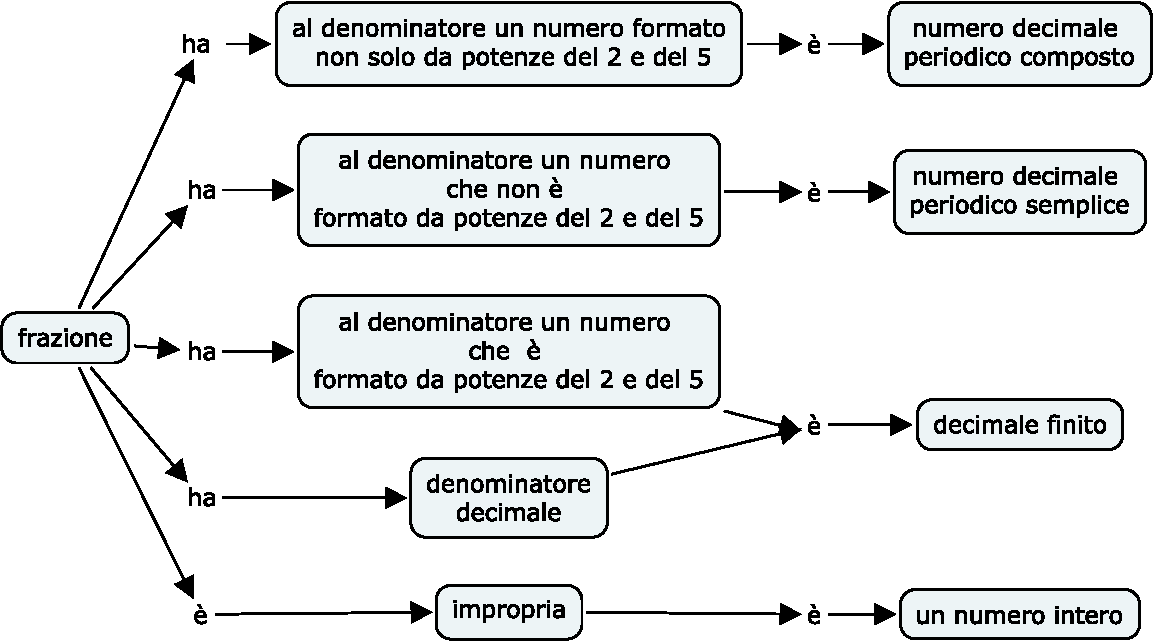
\includegraphics[scale=0.8]{da_frazione_a_numero_decimale-crop}
	\caption{Da frazione a decimale}
	\label{fig:DaFrazioniaDecimale}
\end{figure}
Una frazione è il quoziente di una divisione quindi ad una frazione è associata una divisione. Avremo molti casi fra loro diversi:
\begin{itemize}
	\item La frazione è una frazione apparente. In questo caso ad una frazione corrisponde un numero intero esempio: \[\dfrac{8}{4}=\num{2}\]
	\item La frazione ha per denominatore una potenza del dieci allora alla frazione corrisponde un numero decimale finito esempio:\[\dfrac{3}{10}=\num{0.3}\] 
	\item La frazione ha per denominatore un numero formato da potenze del \num{2} e del \num{5}. In questo caso è possibile trasformare la frazione in una frazione decimale. Esempio: \[\dfrac{3}{8}\] In questo casi si procede in questo modo\begin{enumerate}
		\item Si scompone il denominatore in numeri primi in questo caso $8=2^3$
		\item Si considera la seguente tabella 
		\begin{align*}
		\num{10}&=2\cdot 5\\
		\num{100}&=2^2\cdot 5^2\\
		\num{1000}&=2^3\cdot 5^3\\
		\num{10000}&=2^4\cdot 5^4\\
		\cdots&\cdots
		\end{align*}
		Da cui si vede che $2^3$ moltiplicato per $5^3$ da come risulto \num{1000}. Per cui, applicando al proprietà invariantiva che ci garantisce l'equivalenza delle frazioni abbiamo:\[\dfrac{3}{8}=\dfrac{3}{8}\cdot\dfrac{5^3}{5^3}=\dfrac{375}{1000}=\num{0,375}\] che è un decimale finito.
	\end{enumerate}
	Analogo esempio per \[\dfrac{7}{20}=\dfrac{7}{2^2\cdot 5}=\dfrac{7}{2^2\cdot 5}\cdot\dfrac{5}{5}=\dfrac{35}{100}=\num{0,35}\]
	\item La frazione ha per denominatore un numero non formato da potenze del \num{2} e del \num{5}. Il numero decimale ottenuto è un numero decimale periodico semplice, esempio:\[\dfrac{7}{9}=0{,}77777777\cdots=0{,}\overline{7}\]\[\dfrac{15}{11}=1{,}3636363636\cdots=1{,}\overline{36}\]
	\item La frazione ha per denominatore un numero anche da potenze del \num{2} e del \num{5}. Il numero decimale ottenuto è un numero decimale periodico misto esempio:\[\dfrac{15}{22}=0{,}68181818181818\cdots=0{,}68\overline{18}\]\[\dfrac{33}{14}=2{,}357142857142857\cdots=2{,}357\overline{142857}\]
\end{itemize}
Le parti di un numero decimale hanno un nome che è bene sapere %\[77.825=\overbrace{77}^{\text{parte intera}}.\underbrace{\overline{825}}_{\text{parte decimale}}\]
%\[2.357\overline{142857}=\overbrace{2}^{\text{parte intera}}.\underbrace{\underbrace{357}_{\text{antiperiodo}}\overbrace{\overline{142857}}^{\text{periodo}}}_{\text{parte decimale}} \]
\[\setlength{\tabcolsep}{1pt}
\begin{tabular}{r@{}cccccc}
&&&&\multicolumn{3}{c}{\tiny parte decimale}\\
\addlinespace[-.4ex]
\cmidrule(lr){5-7}
\addlinespace[-1ex]
&&\tiny parte intera&&\tiny antiperiodo&&\tiny periodo\\
\addlinespace[-.4ex]
\cmidrule{3-3}\cmidrule{5-5}\cmidrule{7-7}
\addlinespace[-.4ex]
$2{,}357\overline{142857}$&${}={}$&$2$&,&$357$&&$142857$
\end{tabular}
\]
\subsection{Da numero decimale a frazione}
Possiamo avere due alternative:
\begin{enumerate}
	\item Il numero decimale è un decimale finito. 
	
	Esempi: \numlist{2,3;34,567;0.007} 
	\[\begin{tabular}{ccc}
	$\num{2,3}=\dfrac{23}{10}$&$\num{34.567}=\dfrac{34567}{1000}$&$\num{0.007}=\dfrac{7}{1000}$
	\end{tabular}\]
	Quindi per trovare la frazione generatrice si mette a denominatore il numero senza la virgola e al denominatore una potenza del \num{10} con tanti zeri quanto è lunga la parte decimale.
	\item Il numero decimale è un numero decimale infinito periodico. 
	Esempi: 
	
	\begin{NodesList}
		\centering
		\begin{align*}
		\num{27,49}\overline{932}=\AddNode\\ %[.5cm] 
		=\dfrac{\num{2749932} -\phantom{2749}}{\phantom{99900}}=\AddNode\\[.5cm] %\AddNode[2]\\ 
		=\dfrac{\num{2747932}-\num{2747}}{\phantom{99900}}=\AddNode\\[.5cm]
		=\dfrac{\num{2747932}-\num{2747}}{\num{999}\phantom{00}}=\AddNode\\
		=\dfrac{\num{2747932}-\num{2747}}{\num{99900}}=\AddNode\\
		=\dfrac{\num{2747185}}{\num{99900}}\AddNode
		\end{align*}
		\LinkNodes[margin=3cm]{\begin{minipage}[h]{3.5cm}
				Prendo tutto il numero senza la virgola
			\end{minipage}}
			\LinkNodes[margin=3cm]{\begin{minipage}[h]{3.5cm}
					Sottraggo il numero escluso il periodo
				\end{minipage}}%
				\LinkNodes[margin=3cm]{\begin{minipage}[h]{3.5cm}
						Il periodo è lungo tre divido per $999$
					\end{minipage}}%
					\LinkNodes[margin=3cm]{\begin{minipage}[h]{3.5cm}
							L'antiperiodo è lungo $2$ aggiungo quindi due zeri 
						\end{minipage}}%
						\LinkNodes[margin=3cm]{\begin{minipage}[h]{3.5cm}
								Ottengo
							\end{minipage}}%
						\end{NodesList}
						
\begin{NodesList}
		\centering
		\begin{align*}
		\num{7,4}\overline{25}=\AddNode\\[.5cm] 
		=\dfrac{\num{7425}-\phantom{74}}{\phantom{990}}=\AddNode\\ %[.5cm] %\AddNode[2]\\ 
		=\dfrac{\num{7425}-\num{74}}{\phantom{990}}=\AddNode\\[.5cm]
		=\dfrac{\num{7425}-\num{74}}{\num{99}\phantom{0}}=\AddNode\\
		=\dfrac{\num{7425}-\num{74}}{\num{990}}=\AddNode\\
		=\dfrac{\num{7351}}{\num{990}}\AddNode
		\end{align*}
		\LinkNodes[margin=3cm]{\begin{minipage}[h]{3.5cm}
				Prendo tutto il numero senza la virgola
			\end{minipage}}
			%\LinkNodes{Sposto $2x$ a sinistra e cambio di segno}%
			\LinkNodes[margin=3cm]{\begin{minipage}[h]{3.5cm}
					Sottraggo il numero escluso il periodo
				\end{minipage}}%
				\LinkNodes[margin=3cm]{\begin{minipage}[h]{3.5cm}
						il periodo è lungo due quindi divido per $99$
					\end{minipage}}%
					\LinkNodes[margin=3cm]{\begin{minipage}[h]{3.5cm}
							L'antiperiodo è lungo uno quindi aggiungo uno zero 
						\end{minipage}}%
						\LinkNodes[margin=3cm]{\begin{minipage}[h]{3.5cm}
								Ottengo
							\end{minipage}}%
						\end{NodesList}
	
	\begin{NodesList}
		\centering
		\begin{align*}
		\num{35},\overline{5}=\AddNode\\[.5cm] 
		=\dfrac{\num{355} -\phantom{35}}{\phantom{9}}=\AddNode\\[.5cm] %\AddNode[2]\\ 
		=\dfrac{\num{355}-\num{35}}{\phantom{9}}=\AddNode\\[.5cm]
		=\dfrac{\num{355}-\num{35}}{\num{9}}=\AddNode\\
		%	=\dfrac{\num{2747932}-\num{2747}}{\num{99900}}=\AddNode\\
		=\dfrac{\num{320}}{\num{9}}\AddNode
		\end{align*}
		\LinkNodes[margin=3cm]{\begin{minipage}[h]{3.5cm}
				Prendo tutto il numero senza la virgola
			\end{minipage}}
			\LinkNodes[margin=3cm]{\begin{minipage}[h]{3.5cm}
					Sottraggo il numero escluso il periodo
				\end{minipage}}%
				\LinkNodes[margin=3cm]{\begin{minipage}[h]{3.5cm}
						Il periodo è lungo uno divido per $9$
					\end{minipage}}%
					%	\LinkNodes{\begin{minipage}[h]{3.5cm}
					%	L'antiperiodo è lungo $2$ aggiungo quindi due zeri 
					%		\end{minipage}}%
					\LinkNodes[margin=3cm]{\begin{minipage}[h]{3.5cm}
							Ottengo
						\end{minipage}}%
	\end{NodesList}
	
	\begin{NodesList}
		\centering
		\begin{align*}
		\num{0},\overline{25}=\AddNode\\[.5cm] 
		=\dfrac{\num{25} -\phantom{0}}{\phantom{99}}=\AddNode\\[.5cm] %\AddNode[2]\\ 
		=\dfrac{\num{25}-\num{0}}{\phantom{99}}=\AddNode\\[.5cm]
		=\dfrac{\num{25}-\num{0}}{\num{99}}=\AddNode\\
		%	=\dfrac{\num{2747932}-\num{2747}}{\num{99900}}=\AddNode\\
		=\dfrac{\num{25}}{\num{99}}\AddNode
		\end{align*}
		\LinkNodes[margin=3cm]{\begin{minipage}[h]{3.5cm}
				Prendo tutto il numero senza la virgola
			\end{minipage}}
			\LinkNodes[margin=3cm]{\begin{minipage}[h]{3.5cm}
					Sottraggo il numero escluso il periodo
				\end{minipage}}%
				\LinkNodes[margin=3cm]{\begin{minipage}[h]{3.5cm}
						Il periodo è lungo due divido per $99$
					\end{minipage}}%
					%	\LinkNodes{\begin{minipage}[h]{3.5cm}
					%	L'antiperiodo è lungo $2$ aggiungo quindi due zeri 
					%		\end{minipage}}%
					\LinkNodes[margin=3cm]{\begin{minipage}[h]{3.5cm}
							Ottengo
						\end{minipage}}%
					\end{NodesList}
					
\begin{NodesList}
	\centering
	\begin{align*}
	\num{0},3\overline{47}=\AddNode\\[.5cm] 
	=\dfrac{\num{347} -\phantom{3}}{\phantom{99}}=\AddNode\\[.5cm] %\AddNode[2]\\ 
	=\dfrac{\num{347}-\num{3}}{\phantom{99}}=\AddNode\\[.5cm]
	=\dfrac{\num{347}-\num{3}}{\num{99}\phantom{0}}=\AddNode\\
	=\dfrac{\num{347}-\num{3}}{\num{990}}=\AddNode\\
	=\dfrac{\num{344}}{\num{990}}\AddNode
	\end{align*}
	\LinkNodes[margin=3cm]{\begin{minipage}[h]{3.5cm}
			Prendo tutto il numero senza la virgola
		\end{minipage}}
		\LinkNodes[margin=3cm]{\begin{minipage}[h]{3.5cm}
				Sottraggo il numero escluso il periodo
			\end{minipage}}%
			\LinkNodes[margin=3cm]{\begin{minipage}[h]{3.5cm}
					Il periodo è lungo due divido per $99$
				\end{minipage}}%
				\LinkNodes[margin=3cm]{\begin{minipage}[h]{3.5cm}
						L'antiperiodo è lungo $1$ aggiungo quindi uno zero 
					\end{minipage}}%
					\LinkNodes[margin=3cm]{\begin{minipage}[h]{3.5cm}
							Ottengo
						\end{minipage}}%
	\end{NodesList}
	Per trovare la frazione generatrice bisogna togliere la virgola e sottrarre al numero con la parte periodica compresa il numero senza la parte periodica e dividere per un numero composto da tanti nove per quanto è lungo il periodo e tanti zero per quanto è lungo l'antiperiodo. Il perché di questa regola può essere spiegato con questi esempi:
	\begin{enumerate}
		\item Per trovare la funzione generatrice di $x=7{,}2\overline{4}$ si procede in questo modo
		\begin{align*}
		%x=&7{,}2\overline{4}\\
		100x &=724{,}\overline{4}\\
		10x &=72{,}\overline{4}\\
		100x-10x&=724{,}\overline{4}-72{,}\overline{4}=652\\
		90x&=652\\
		x&=\dfrac{652}{90}
		\end{align*}
		\item Per trovare la funzione generatrice di $x=1{,}\overline{2}$ si procede in questo modo
		\begin{align*}
		%	x=&1{,}\overline{2}\\
		10x &=12{,}\overline{2}\\
		x &=1{,}\overline{2}\\
		10x-x&=12{,}\overline{2}-1{,}\overline{2}=11\\
		9x&=11\\
		x&=\dfrac{11}{9}
		\end{align*}
		\item Per trovare la funzione generatrice di $x=1{,}\overline{22}$ si procede in questo modo
		\begin{align*}
		%	x=&1{,}\overline{22}\\
		100x &=122{,}\overline{22}\\
		x &=1{,}\overline{22}\\
		100x-x&=122{,}\overline{22}-1{,}\overline{22}=121\\
		99x&=121\\
		x&=\dfrac{121}{99}
		\end{align*}
	\end{enumerate}
	
\end{enumerate}
Un piccolo gioco 
\[0{,}\overline{9}=1\]
\subsection{Da numero percentuale a decimale}
Per trasformare un numero percentuale in numero decimale basta dividere il numero per cento. 

Esempi:\[10\%= 10:100=0,1 \] \[82,5\%= 82,5:100=0,825 \]
\subsection{Da numero decimale a percentuale}
Per trasformare un numero decimale in percentuale basta moltiplicare il numero per $\dfrac{100}{100}$

Esempio \[\num{4,5}=4,5\cdot\dfrac{100}{100}=\dfrac{450}{100}=450\%\]
\[\num{0,58}=0{,}58\cdot\dfrac{100}{100}=\dfrac{58}{100}=58\%\]
\subsection{Da percentuale a frazione}
Per trasformare una percentuale in una frazione basta ricordare che una percentuale è una divisione per cento.
Esempio
\[20\%=\dfrac{20}{100} \]
\subsection{Da frazione a percentuale}
La trasformazione è in due tempi 
\begin{enumerate}
	\item Trasformo la frazione in un numero decimale
	\item Trasformo il numero decimale in percentuale
\end{enumerate}
Esempio 
\[\dfrac{75}{4}=18,75=18,75\cdot\dfrac{100}{100}=1875\% \]

\section{Frazioni equivalenti}
\label{sec:FrazioniEquivalentiNumRazzASS}
Due frazioni sono equivalenti quando rappresentano lo stesso quoziente. Esempio  $\dfrac{3}{4}$ e $\dfrac{6}{8}$ sono equivalenti e  si scrive \[\dfrac{2}{3} \equiv\dfrac{6}{8}\]

Se due frazioni sono equivalenti vale il cosiddetto prodotto in croce e viceversa, cioè:
\begin{center}
\prodcroce{A}{B}{C}{D}
\end{center}
Esempio 
%\begin{document}
\begin{center}
\prodcroce{3}{4}{6}{8}
\end{center}
quindi le due frazioni sono equivalenti
\section{Proprietà  invariantiva}
\label{sec:propInvariantivaNumASS}

Moltiplicando o dividendo per un numero diverso da zero il numeratore e il denominatore di una frazione si ottiene una frazione equivalente 
infatti $\dfrac{a}{b}=\dfrac{ac}{bc}$
\begin{center}
 \prodcroce{a}{b}{ac}{bc}
\end{center}

Esempio

\[\dfrac{3}{4}=\dfrac{3\cdot 8}{4\cdot 8}=\dfrac{24}{32}\]   le due frazioni sono equivalenti infatti: 

\[\prodcroce{3}{4}{24}{32}\]

Esempio:

\[\dfrac{6}{8}=\dfrac{6:2}{8:2}=\dfrac{3}{4}\]   le due frazioni sono equivalenti infatti: 

\[\prodcroce{6}{8}{3}{4}\]
\section{Semplificare una frazione}
\label{sec:sempunaFrazASS}
Semplificare una frazione significa dividere il numeratore e il denominatore per il loro Massimo Comune Divisore (MCD). Per la proprietà invariantiva la frazione ottenuta è equivalente a quella data.
La procedura è quindi la seguente 

Data la frazione $\dfrac{a}{b}$

\begin{enumerate}
	\item Calcolo il $\mcd(a,b)$
	\item Divido il numeratore e il denominatore per  $\mcd(a,b)$
\end{enumerate}

Esempio 

Semplificare la frazione $\dfrac{84}{48}$  
\begin{enumerate}
	\item Inizio con  trovare il $\mcd(84,48)$ li scompongo in fattori primi e ottengo
	
	\begin{center}
	\begin{tabular}{cc}
		\primedecomp{84}&\primedecomp{48}\\
		$48 =2^4\cdot  3$&	$84=2^2\cdot 3\cdot 7$
	\end{tabular}
	\end{center}
	quindi $\mcd(84,48)=2^2\cdot 3=12$
	\item 	Divido numeratore e denominatore per 12 e ottengo $\dfrac{7}{4}$
\end{enumerate}
	Vi è un altro metodo per semplificare una frazione: Dividere se possibile numeratore e denominatore per uno stesso numero e continuare finché ciò è possibile come nell'esempio successivo.
	
	\begin{center}
	\begin{tikzpicture}[thick]
	\node at (0,0) {$\displaystyle \dfrac{84}{48}$};
	\node at (0.5,0.5) {$\displaystyle 42$};
	\node at (0.5,-0.5) {24};
	\node at (1,0.6){21};
	\node at (1,-0.6){12};
	\node at (1.4,0.7){7};
	\node at (1.4,-0.7){4};
	\end{tikzpicture}
	\end{center}
	%$\dfrac{\cancel{84}}{\cancel{48}}\rightarrow\dfrac{\cancel{42}}{\cancel{24}}\rightarrow\dfrac{\cancel{21}}{\cancel{12}}\rightarrow\dfrac{7}{4} $
	\section{Riduzione allo stesso denominatore}
	\label{sec:RiduzionestessoindiceFrazzASS}
	La proprietà invariantiva permette di trasformare due frazioni a denominatore diverso in due frazioni che hanno lo stesso denominatore.
	Il procedimento è il seguente 
	\begin{enumerate}
		\item Date le frazioni $\dfrac{5}{21}$ e $\dfrac{7}{12}$
		\item Scompongo i denominatori in fattori primi cioè:
		
		\begin{center}
			\begin{tabular}{cc}
				\primedecomp{21}&\primedecomp{12}\\
				$21=3\cdot 7$& $12=3\cdot 2^4$
			\end{tabular}
		\end{center}
	    \item Calcolo il $\mcm$ che in questo caso è $\mcm(21,12)=2^2\cdot 3\cdot 7=84$ 		
		\item Scrivo due frazioni con denominatore 84 cioè $\dfrac{}{84}$ e $\dfrac{}{84}$
		\item Applico la proprietà invariantiva al numeratore e scrivo $\dfrac{84:21\cdot 5}{84}$ e $\dfrac{84:12\cdot 7}{84}$
		\item Otteniamo $\dfrac{20}{84}$ e $\dfrac{49}{84}$
	\end{enumerate}
	\subsection{Confronto fra frazioni}
	Per confrontare due frazioni le riduco allo stesso denominatore è maggiore la frazione con denominatore maggiore.
	
	Esempio Ordinare in modo decrescente le seguenti frazioni
	\begin{align*}
		&\dfrac{1}{2}&\dfrac{1}{3}&&\dfrac{3}{5}&&\dfrac{3}{8}\\
		\text{Calcolo il mcm}\\
		&\dfrac{}{120}&\dfrac{}{120}&&\dfrac{}{120}&&\dfrac{}{120}\\
		\text{Riduco allo stesso denominatore}\\
		&\dfrac{60}{120}&\dfrac{40}{120}&&\dfrac{72}{120}&&\dfrac{45}{120}\\
	\end{align*}

		La frazione che ha il numeratore più grande è $\dfrac{72}{120}$ che corrisponde a $\dfrac{3}{5}$ questa è la frazione più grande. A questa
		segue $\dfrac{3}{8}$ perché corrisponde a $\dfrac{45}{120}$ e così di seguito $\dfrac{1}{2}$ ed infine $\dfrac{1}{3}$.
%\mediapriorita{Aggiungere esempi}
	\section{Operazioni}
	\label{sec:OperazioniASS}
	\subsection{Somma e sottrazione}
	\label{ssec:SommaesottrazioniASS}
	Nel sommare due frazioni possiamo avere due casi 
	\begin{enumerate}
		\item Denominatori uguali
		
		La somma/differenza due frazioni che hanno lo stesso denominatore è una frazione che ha lo stesso denominatore e per numeratore la somma/differenza dei numeratori. 
		
		Esempio: \[\dfrac{2}{3}+\dfrac{8}{3}=\dfrac{10}{3}\] Esempio \[\dfrac{12}{5}-\dfrac{8}{5}=\dfrac{4}{5}\]
		\item Denominatori diversi
		
		Riduco le due frazioni allo stesso denominatore come in\nobs\vref{sec:RiduzionestessoindiceFrazzASS} e quindi sommo.
		
		Esempio:\begin{align*}
		&\dfrac{2}{3}+\dfrac{7}{5}\\
		&\text{Calcolo}\\
		&\mcd(3,5)=15\\
		&\dfrac{15:3\cdot 2+15:5\cdot 7}{15}\\
		&\dfrac{10+21}{15}\\
		&\dfrac{21}{15}
		\end{align*}
	\end{enumerate}
	\begin{table}
		\centering
		\begin{tikzpicture}[auto, -stealth, thick, scale=0.5]
		% Definizione dei nodi e delle loro scatole
		\tikzstyle{line} = [draw, -latex']
		\node[ellipse, minimum height=4em, draw, very thick,inner xsep=3em] at (0,0) (primo) {Inizio};
		\node[rectangle,minimum height=4em,draw, very thick, text width=5cm,align=flush center] at (0,-5) (secondo) {Calcola mcm fra i denominatori};
		\node[rectangle,minimum height=4em,draw, very thick, text width=5cm,align=flush center] at (0,-11
		) (terzo) {Dividi il mcm per denominatore e moltiplico il risultato per il numeratore};
		\node[diamond,aspect=2,draw, very thick,inner xsep=3em, text width=2cm,align=flush center] at (0,-18) (quarto){ le frazioni sono finite?};
		\node[rectangle,minimum height=4em,draw, very thick, text width=5cm,align=flush center] at (0,-25) (quinto) {Somma i valori trovati};  		
		
		\node[ellipse ,minimum height=4em,draw, very thick,inner xsep=3em] at (0,-29) (sesto) {Fine};
		% collegamento dei nodi
		\begin{scope}[every path/.style=line]
		\path  (primo) --  (secondo);
		\path (secondo) edge  (terzo);
		\path (terzo)--(quarto);
		\path (quarto)  -- node  {SI} (quinto);
		\path (quarto.west)  -|  node [near start] {NO}+(-5em,0) |- (terzo);
		\path(quarto)--(quinto);
		\path(quinto)--(sesto);
		\end{scope}
		\end{tikzpicture}
		\caption{Somma di frazioni}
		\label{tab:sommadifrazioniASS}
	\end{table}
	\subsection{Moltiplicazione}
	\label{sec:MoltiplicazioneASS}
	Nel moltiplicare  due frazioni possiamo avere due casi 
	\begin{enumerate}
		\item frazione con frazione
		
		Esempio \begin{center}
					\begin{tikzpicture}[thick]
					\def\x{2.8mm}
					\def\h{2.4mm}
					\def\dist{10mm}%1cm
					\node at (0,0) {$\displaystyle \dfrac{21}{4}$};
					\node at (\dist,0) {$\displaystyle \dfrac{3}{5}$};
					\node at (\dist/2,0) {$\cdot$};
					\node  at (-\dist,0) {$\displaystyle \dfrac{21}{4}\cdot\displaystyle \dfrac{3}{5}= $};
					\draw[-stealth] (\x, -\h)--(\dist-\x,-\h);
					\draw[-stealth] (\x,\h)--(\dist -\x, \h);
					\node at (2.2*\dist,0) {$=\displaystyle \dfrac{21\cdot 3}{4\cdot 5}=\displaystyle \dfrac{63}{20}$};
					% \draw[-stealth] (-\x,\h)--(-\x, -\h);
					%   \draw[-stealth] (\dist+\x,\h)--(\dist+\x, -\h);
					\end{tikzpicture}%
		\end{center}
		
		quindi nella moltiplicazione fra due frazioni si  moltiplicano numeratore con numeratore e denominatore con denominatore.
		\item frazione con numero
	   
	   Esempio
	   
	   \begin{center}
	 \begin{tikzpicture}[thick]
	 \def\x{2.8mm}
	 \def\h{2.4mm}
	 \def\dist{10mm}%1cm
	 \node  at (-\dist,0) {$\displaystyle \dfrac{5}{4}\cdot 7 = $};
	 \node at (0,0) {$\displaystyle \dfrac{5}{4}$};
	 \node at (\dist,0) {$\displaystyle \dfrac{7}{1}$};
	 \node at (\dist/2,0) {$\cdot$};
	 
	 %	\draw[-stealth] (\x, -\h)--(\dist-\x,-\h);
	 \draw[-stealth] (\x,\h)--(\dist -\x, \h);
	 \node at (2.2*\dist,0) {$=\displaystyle \dfrac{5\cdot 7}{4}=\displaystyle \dfrac{35}{4}$};
	 % \draw[-stealth] (-\x,\h)--(-\x, -\h);
	 %   \draw[-stealth] (\dist+\x,\h)--(\dist+\x, -\h);
	 \end{tikzpicture}%
	   \end{center}
	   quindi nella moltiplicazione fra una frazione e un numero si moltiplica il numero con il numeratore e il denominatore resta uguale.
	\end{enumerate}
	\subsection{Semplificazioni e moltiplicazioni}
	Semplificare una frazione è possibile quando numeratore e denominatore sono divisibili per lo stesso numero. La semplificazione avviene quindi in verticale come per esempio:
	\begin{center}
		\begin{tikzpicture}[thick]
		\def\x{2.8mm}
		\def\h{2.4mm}
		\node at (0,0) {$\displaystyle \dfrac{4}{16}$};
		\node at (\x+15,0) {$\displaystyle= \dfrac{1}{4}$};
		\draw[-stealth] (-\x,\h)--(-\x, -\h);
		\draw[-stealth] (\x,\h)--(\x, -\h);
		\end{tikzpicture}%
	\end{center}
	
	Con la moltiplicazione è possibile anche la cosiddetta semplificazione\index{Semplificazione!in croce} in croce come per esempio: 
	         \begin{center}
	         	\begin{tikzpicture}[thick]
	         	\def\x{2.8mm}
	         	\def\h{2.4mm}
	         	\def\dist{12mm}%1cm
	         	\node at (0,0) {$\displaystyle \dfrac{5}{27}$};
	         	\node  at(-0.5,0.5) {1};
	         	\node  at(-0.5,-0.5) {3};
	         	\node at (\dist,0) {$\displaystyle \dfrac{9}{20}$};
	         	\node at (2*\dist+\x,0) {$\displaystyle =\dfrac{1\cdot 1}{3\cdot 4}=\dfrac{1}{12}$};
	         	\node at (\dist+10,0.5){1};
	         	\node at (\dist+10,-0.5){4};
	         	\draw[-stealth] (\x, \h)--(\dist-\x,-\h);
	         	\draw[-stealth] (\x,-\h)--(\dist -\x, \h);
	         	%\draw[-stealth] (-\x,\h)--(-\x, -\h);
	         	%\draw[-stealth] (\dist+\x,\h)--(\dist+\x, -\h);
	         	\end{tikzpicture}%
	         \end{center}	
	
	
	In questo caso è possibile semplificare il denominatore della prima frazione con il numeratore della seconda e il numeratore della prima con il denominatore della seconda.

\subsection{Divisione fra frazioni}

Prima di parlare di divisioni fra frazioni occorre parlare di reciproci. Due numeri sono reciproci\index{Numero!reciproco} se il loro prodotto è uno. Quindi per le frazioni avremo per esempio:\[\dfrac{2}{5}\cdot\dfrac{5}{2}=1\]In questo caso si dice che $\dfrac{2}{5}$ e $\dfrac{5}{2}$ sono frazioni fra loro reciproche.
Per un numero intero avremo per esempio\[2\cdot\dfrac{1}{2}=1\]

In pratica  avremo che per trovare il reciproco di un numero avremo due casi
\begin{enumerate}
	\item Il numero è una frazione. In questo caso basta scrivere una frazione con numeratore e denominatore scambiato fra loro.
	\item Il numero è un numero intero. In questo caso basta scrivere una frazione che ha per numeratore uno e per denominatore il numero di partenza 
\end{enumerate}

Per dividere due frazioni bisogna trasformare la divisione nel prodotto della prima per il reciproco della seconda. Esempio

\[\dfrac{7}{4}:\dfrac{4}{5}=\dfrac{7}{4}\cdot\dfrac{5}{4}=\dfrac{7\cdot 5}{5\cdot 4}=\dfrac{35}{20}\]

Se divido una frazione per un numero, trasformerò la divisione nella moltiplicazione della frazione per il reciproco del numero.

\[\dfrac{7}{4}:3=\dfrac{7}{4}\cdot\dfrac{1}{3}=\dfrac{7\cdot 1}{4\cdot 3}=\dfrac{7}{12} \]
\subsection{Potenze}

La potenza di una frazione è uguale alla potenza del numeratore fratto la potenza del denominatore.
\[\left( \dfrac{3}{2}\right)^3=\dfrac{3^3}{2^3}=\dfrac{27}{8} \]

